\documentclass[border=2mm]{standalone}
\usepackage{amsmath}
\usepackage{tikz}
\usetikzlibrary{arrows.meta,positioning,calc}
% SCHEME COLOR: one mid-grey for both GitHub light and dark themes
\definecolor{schemeink}{HTML}{808080}
\tikzset{every picture/.append style={color=schemeink}}
\newcommand{\hzero}{\mathbf{h}_0}
\newcommand{\hone}{\mathbf{h}_1}
\newcommand{\Lzero}{L_0}
\newcommand{\Lone}{L_1}
\newcommand{\etazero}{\eta_0}
\newcommand{\etaone}{\eta_1}
\begin{document}
% Alternative A — Minimal / academic (Forney-style) — Fig 2 partner.
% Compactness pass: min height 9mm, min width 15mm (FIR) / 11mm (gain), inner sep 4pt.
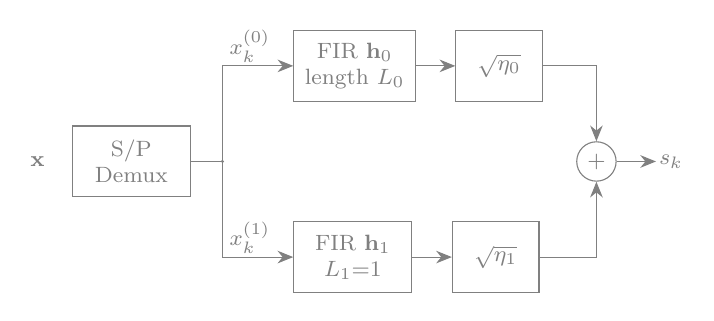
\begin{tikzpicture}[
  >={Stealth[length=2mm,width=1.6mm]},
  every path/.style={line width=0.4pt},
  block/.style={draw, line width=0.4pt,
                minimum height=9mm, minimum width=15mm,
                inner sep=4pt, align=center, font=\footnotesize},
  gainblk/.style={draw, line width=0.4pt,
                  minimum height=9mm, minimum width=11mm,
                  inner sep=4pt, align=center, font=\footnotesize},
  sumnode/.style={draw, circle, line width=0.4pt, inner sep=0pt,
                  minimum size=5mm, font=\footnotesize},
  signal/.style={font=\footnotesize, inner sep=1pt},
]
% --- Input + demultiplexer ---
\node[signal] (x) {$\mathbf{x}$};
\node[block, right=3mm of x] (demux) {S/P\\Demux};

% Branching tee just right of demux
\coordinate (tee) at ($(demux.east)+(4mm,0)$);
\draw (demux.east) -- (tee);

% --- Stream 0 (top): FIR h_0, length L_0, scaled by sqrt(eta_0) ---
\node[block,   above right=3mm and 13mm of demux] (h0) {FIR $\hzero$\\length $\Lzero$};
\node[gainblk, right=5mm of h0]                   (g0) {$\sqrt{\etazero}$};

% --- Stream 1 (bottom): FIR h_1, length L_1=1, scaled by sqrt(eta_1) ---
\node[block,   below right=3mm and 13mm of demux] (h1) {FIR $\hone$\\$\Lone{=}1$};
\node[gainblk, right=5mm of h1]                   (g1) {$\sqrt{\etaone}$};

% --- Summation and output ---
\node[sumnode, right=10mm of $(g0)!0.5!(g1)$] (sum) {$+$};
\node[signal,  right=5mm of sum]              (s)   {$s_k$};

% Branching arrows from tee into h0 / h1; stream labels sit on the horizontal
% lead-in a few mm clear of the FIR blocks so they never touch the boxes.
\draw[->] (tee) |- (h0.west);
\draw[->] (tee) |- (h1.west);
\node[signal, above] at ($(h0.west)+(-5.5mm,0)$) {$x^{(0)}_k$};
\node[signal, above] at ($(h1.west)+(-5.5mm,0)$) {$x^{(1)}_k$};
\fill (tee) circle (0.6pt);

% Stream-internal arrows
\draw[->] (h0) -- (g0);
\draw[->] (h1) -- (g1);

% Merge into summation node
\draw[->] (g0.east) -| (sum.north);
\draw[->] (g1.east) -| (sum.south);
\draw[->] (sum) -- (s);
\end{tikzpicture}

\end{document}
